\documentclass{article}
\usepackage[utf8]{inputenc}
\usepackage{listings}
\usepackage{xcolor}
\usepackage{graphicx}
\usepackage{hyperref}

\title{Assignment02}
\author{zitian wang}
\date{\today}

\lstset{
  language=Java,
  basicstyle=\ttfamily\small,
  keywordstyle=\color{blue}\bfseries,
  stringstyle=\color{red},
  commentstyle=\color{gray},
  numbers=left,
  numberstyle=\tiny\color{gray},
  stepnumber=1,
  numbersep=10pt,
  tabsize=4,
  showstringspaces=false,
  breaklines=true,
  frame=single
}

\begin{document}

\maketitle

\section{Android Basics}
\subsection{What does the “android:minSdkVersion” in android project indicate?}
The `android:minSdkVersion` in an Android project specifies the minimum API level (version of the Android operating system) required to run the app. It ensures compatibility, meaning the app will not install or run on devices with a lower API level than specified. 

\subsection{Why Android documentation indicates that declaring the attribute “android:
maxSdkVersion” is not recommended?}
Declaring the `android:maxSdkVersion` attribute is not recommended because it sets an upper limit on the API level that the app can run on. This restricts the app from being installed on newer Android versions beyond the specified maximum. As Android evolves, backward compatibility is generally maintained, so limiting the app to specific API levels unnecessarily restricts its reach and prevents it from benefiting from future updates and improvements in the Android ecosystem. Instead, it is better to test for compatibility with newer versions as they are released.

\subsection{What are the two types of Navigation Drawer? Explain the differences between the two types?}
There are two types of Navigation Drawers in Android:
\begin{enumerate}
    \item \textbf{Standard Navigation Drawer}: 
    A full-screen drawer that is attached to the edge of the screen and can either push or overlap the content when opened. It is generally used for primary navigation in apps with multiple sections.
    
    \item \textbf{Modal Navigation Drawer}:
    A floating drawer that slides over the app content, often dimming the background to draw focus. It is suitable for simpler navigation or scenarios where the context of the current screen should be maintained.
\end{enumerate}

The key difference lies in how the drawers interact with the screen content: the Standard Drawer integrates with the full screen, while the Modal Drawer appears as an overlay, offering distinct user interaction experiences.

\section{Material Design}
\subsection{Change the icon of the app}
Because the app is ralative to running, so set a shoes as its icon.

\begin{figure}[h]
    \centering
    
\includegraphics[width=0.2\textwidth]{./pictures/running-shoes.png}
    \caption{Icon of a App}
    \label{fig:example}
\end{figure}

\subsection{Dark theme}
Based on the information provided in the previous course, there are a number of design websites that can directly produce the app's corresponding light and dark theme files. Since I didn't know that the colors of the original example code were based on that theme, I chose to add another color of cleanser as the night theme.
\begin{figure}[h]
    \centering
    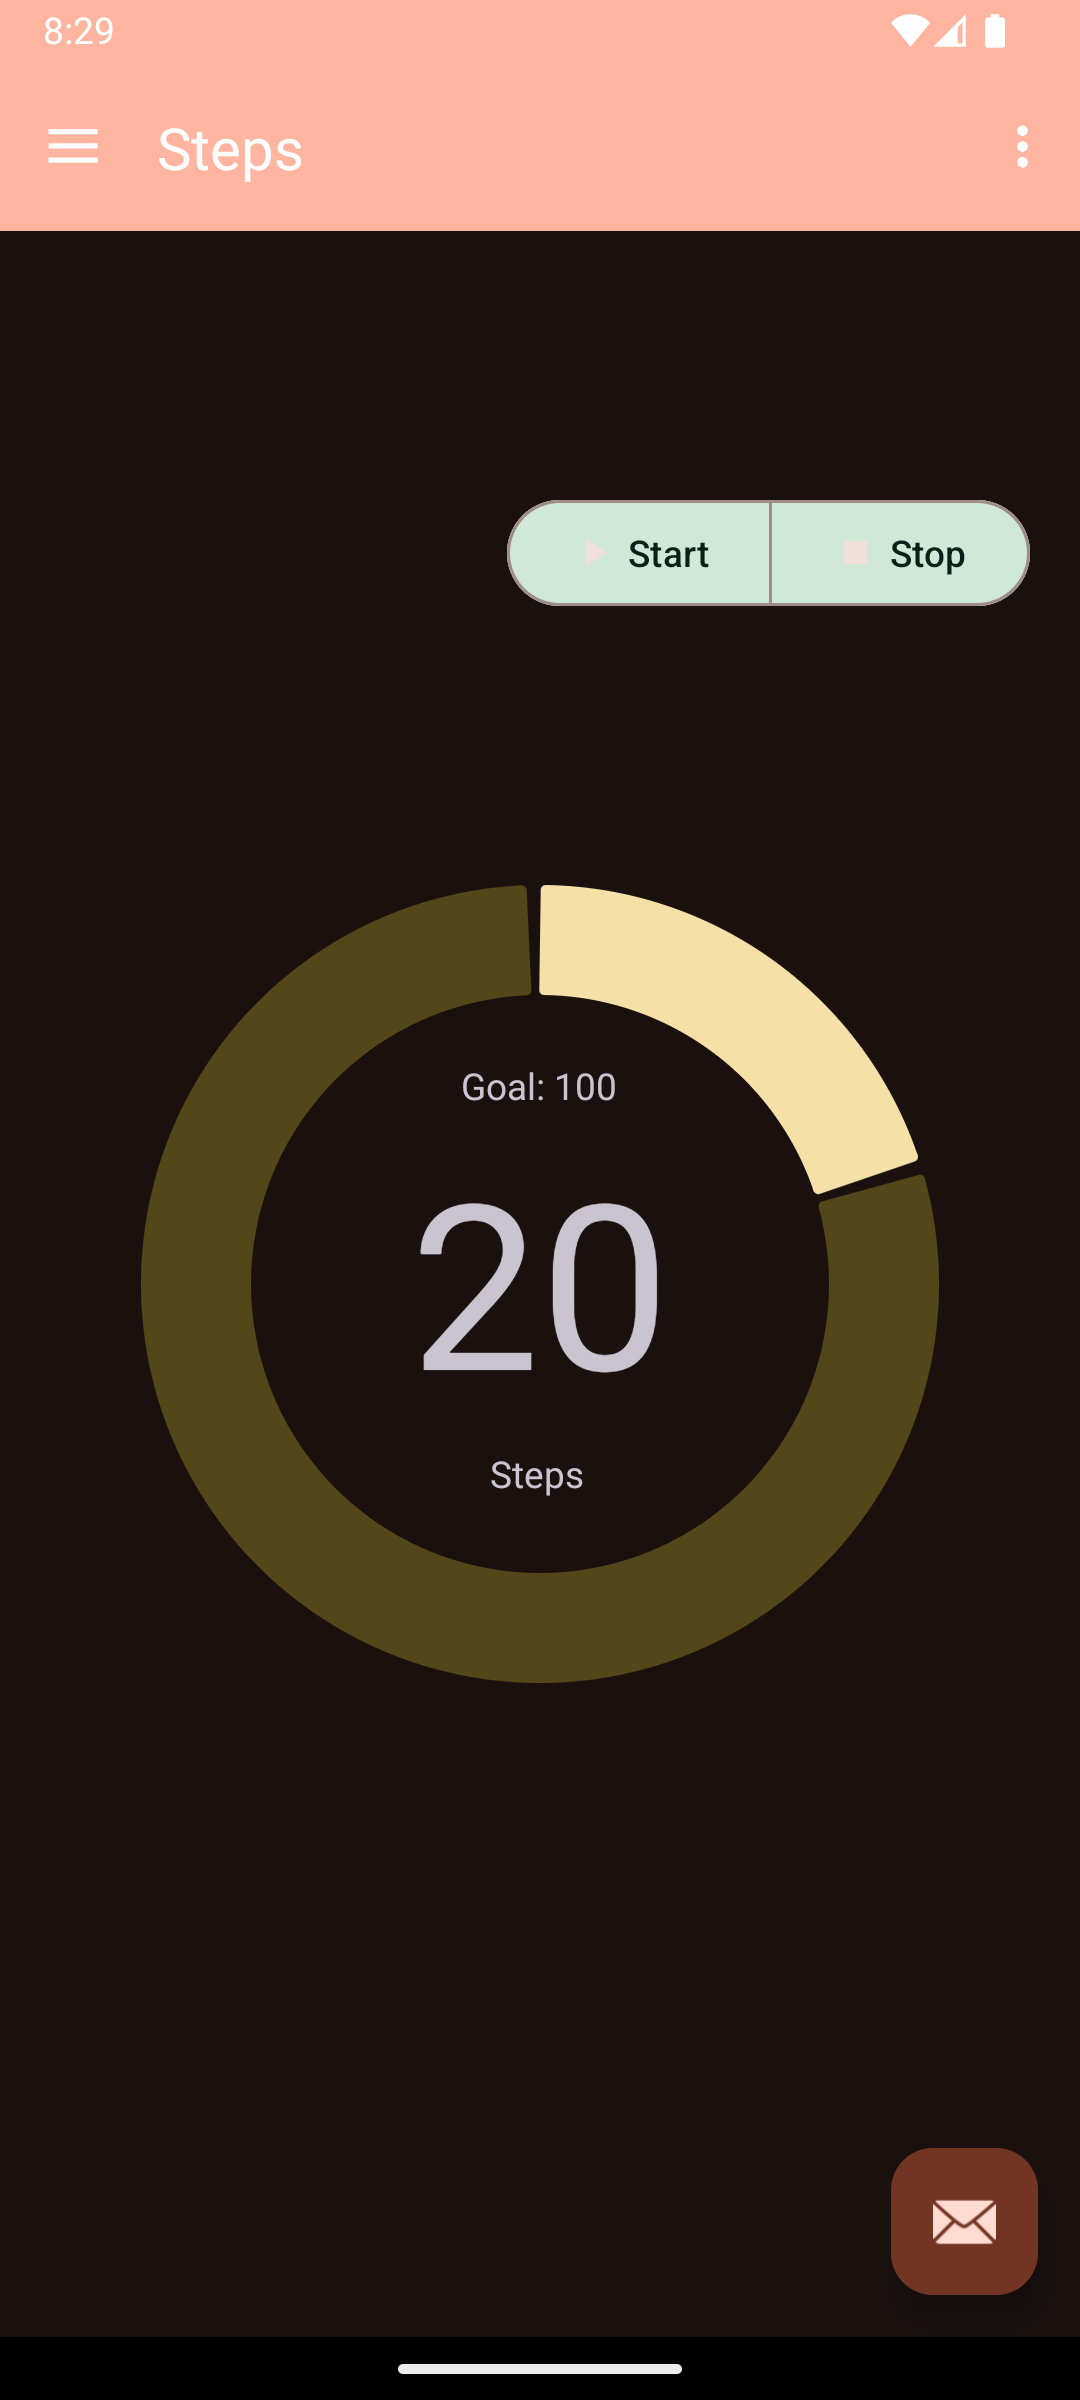
\includegraphics[width=0.2\textwidth]{./pictures/darkTheme.png}
    \caption{Dark theme}
    \label{fig:example}
\end{figure}

The implementation involves adding two files, \texttt{color.xml} and \texttt{theme.xml}, in the \texttt{values-night} directory to configure the desired colors for night mode. It is important to ensure that any changes made to the color definitions in this directory are synchronized with the corresponding \texttt{color.xml} file in the \texttt{values} directory. This guarantees consistency between the color schemes used for both the standard and night modes, providing a cohesive user experience.

\section{Step Counter}
The countSteps() function implements part of the function by controlling the refresh time to avoid system crash, and the \texttt{handler.post()} method ensures that the interface can be updated in a timely manner.
\begin{lstlisting}
private void countSteps(float step) {
    accStepCounter += step;
    long currentTime = System.currentTimeMillis();


    if (currentTime - lastUpdate > 1000) {
        lastUpdate = currentTime;

        handler.post(() -> {
            if (progressBar != null) {
                progressBar.setProgress(accStepCounter);
            }
            if (stepCountsView != null) {
                stepCountsView.setText(String.valueOf(accStepCounter));
            }
        });


        Log.d("STEP DETECTOR STEPS: ", String.valueOf(accStepCounter));
        saveStepInDatabase();
    }
}
\end{lstlisting}
The calling function part of the code is as follows:
\begin{lstlisting}
case Sensor.TYPE_STEP_DETECTOR:
    countSteps(sensorEvent.values[0]);
    break;
\end{lstlisting}
The functions for importing data from the database are as follows:
\newpage
\begin{lstlisting}
private void loadSingleRecord() {
    SimpleDateFormat sdf = new SimpleDateFormat("yyyy-MM-dd");
    String currentDate = sdf.format(System.currentTimeMillis());

    int steps = StepAppOpenHelper.loadSingleRecord(getActivity(), currentDate);

    if (progressBar != null) {
        progressBar.setProgress(steps);
    }
    if (stepsTextView != null) {
        stepsTextView.setText(String.valueOf(steps));
    }
    stepsCounter = steps;
}
\end{lstlisting}
Since the simulator is not convenient to simulate the corresponding sensors, the debugging of the code is done on the Android phone.
\begin{figure}[h]
    \centering
    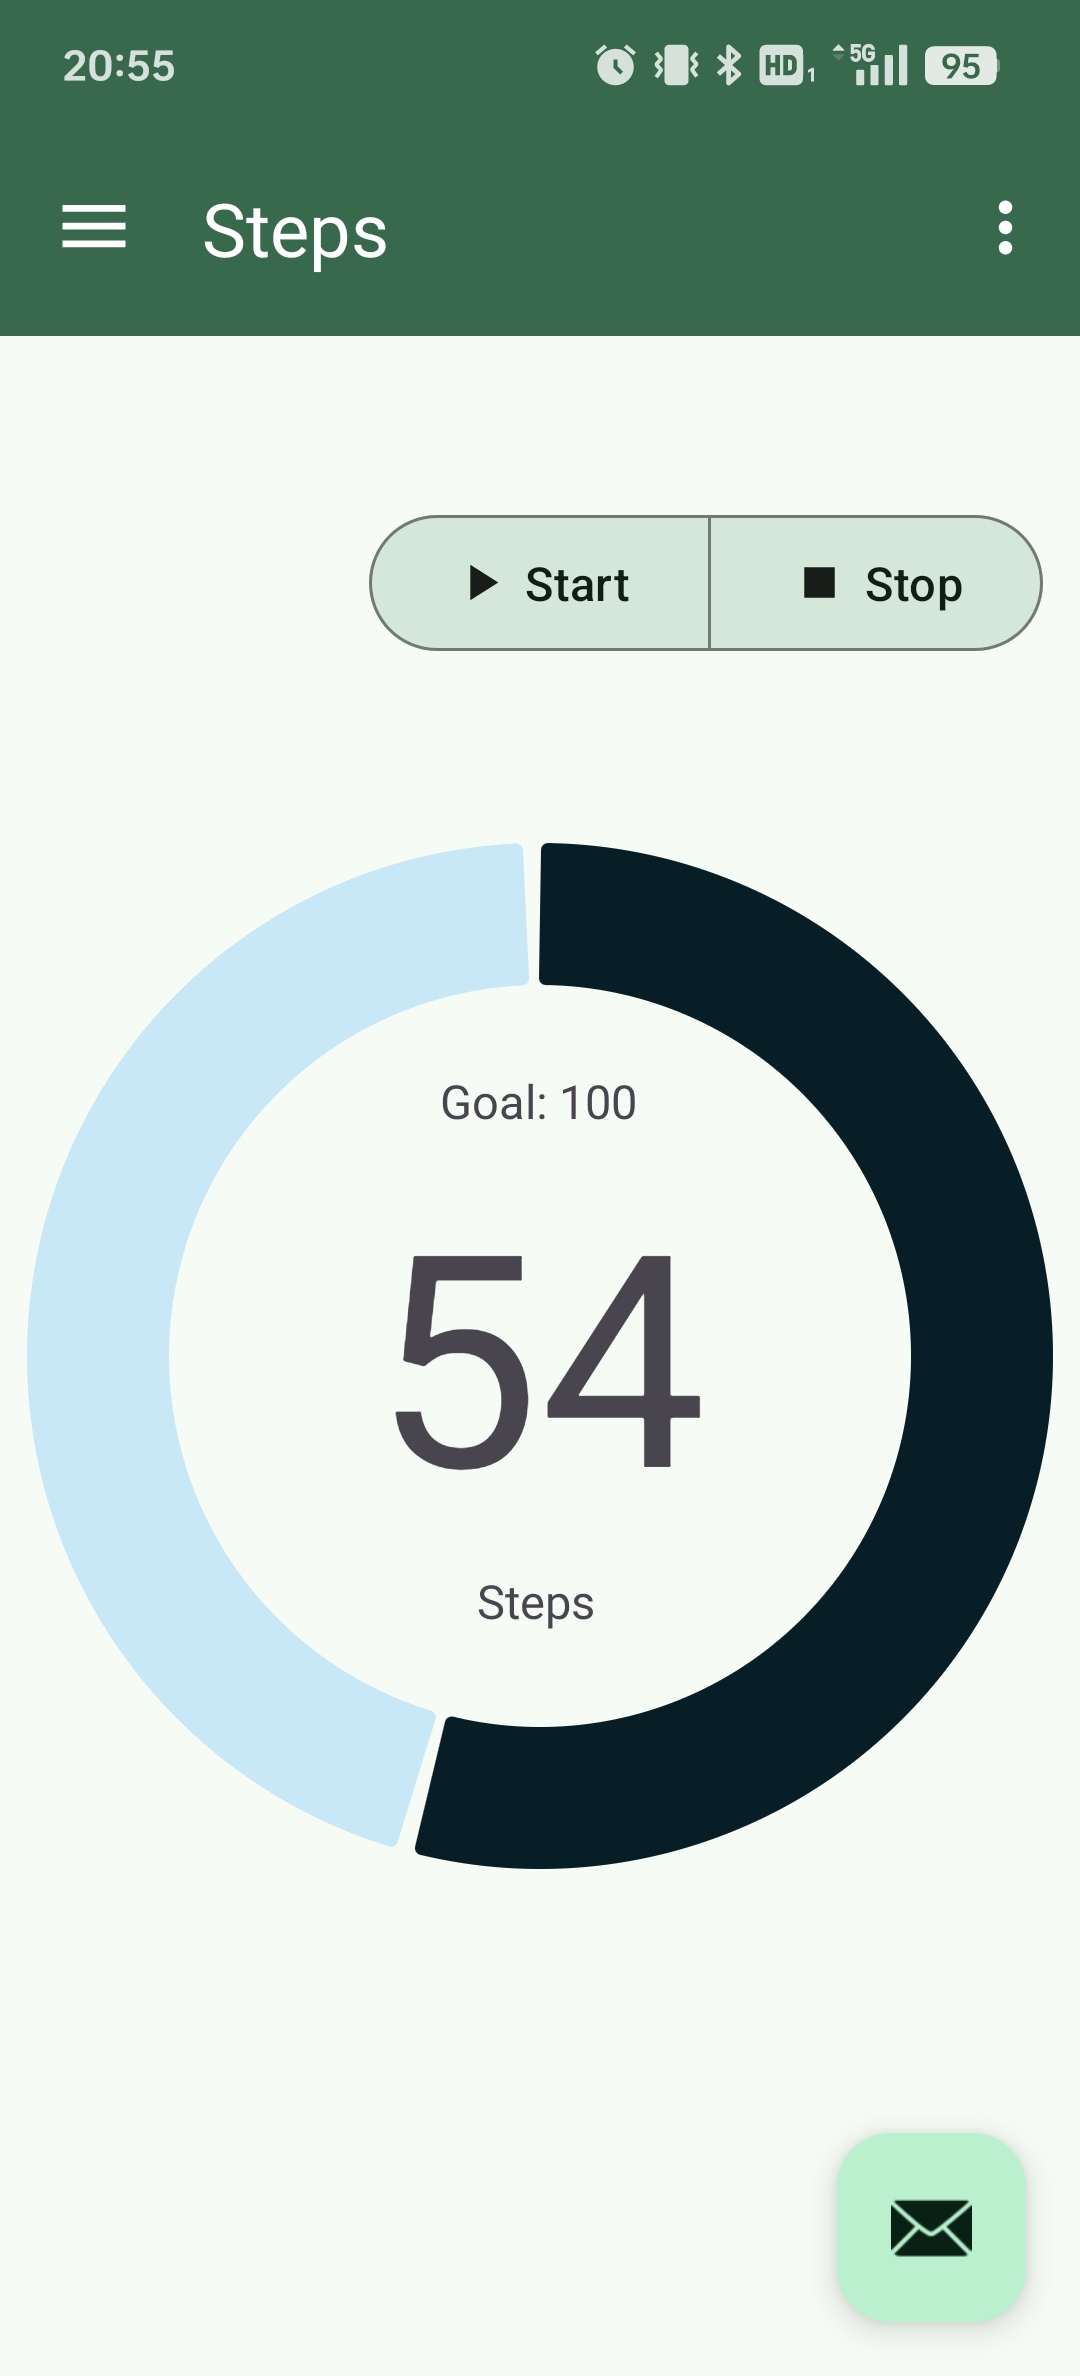
\includegraphics[width=0.3\textwidth]{./pictures/debug.png}
    \caption{Live demo}
    \label{fig:example}
\end{figure}
The main code changes have been listed in the report, check the github repository for details.
\href{https://github.com/ZenWang00/Mobile-and-Wearable-Computing-SA-2024-2025/tree/main/MWC-StepAppV4-Startup-Code/StepAppV4}{StepAppV4 GitHub Repository}
\end{document}
